\documentclass{article}

\title{Computer Architecture (From the Ground Up)}
\author{Nicoll Douglas}

\usepackage{float}

\usepackage{graphicx}
\graphicspath{ {./images/} }

\usepackage{xcolor}
\definecolor{linkColor}{RGB}{0, 102, 204}

\usepackage[colorlinks=true]{hyperref}
\hypersetup{
    linkcolor=linkColor
}

\usepackage[toc, hyperfirst=true]{glossaries-extra}
\setabbreviationstyle{long-short-desc}
\makeglossaries
\loadglsentries{glossary.tex}

\begin{document}
\maketitle
\tableofcontents

\section{Electronics Theory}

\subsection{Electric Force}

\subsubsection{What is Charge?}

Charge is a fundamental property of matter that causes it to experience a force when placed in an electric or magnetic field (electromagnetic field). Protons carry a positive charge, electrons carry a negative charge, neutrons carry no charge. Opposite charges will pull each other together, like charges will push away from each other.

Simple, singular, stationary protons and electrons have an electric field. A proton has an electric field that points outwards in all directions. An electron has an electric field that points inwards in all directions. They do not have a magnetic field.

\begin{figure}[H]
    \centering
    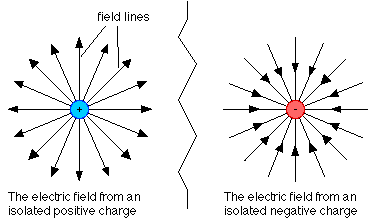
\includegraphics[width=0.7\textwidth]{isolated_electric_fields.png}
    \caption{The electric fields of a single, stationary proton and electron}
\end{figure}

\subsubsection{What is an Electric Field?}

An electric field is an invisible area of influence surrounding an electrically charged object such as a proton or electron. The direction of an electric field is the direction a positive charge would be pushed.

When a proton is put nearby an electron (i.e \emph{placed in its electric field}), the electric fields overlap to create a singular electric field. They will \emph{naturally} pull towards each other (a consequence of charge). The opposite occurs when two particles of the same charge are put next to each other meaning they will push away from each other. This pushing/pulling is known as the \textbf{electrostatic force} when the particles are standing still and more broadly as the \textbf{electric} force since the charges or stationary or moving. The push Each particle experiences a force that is exerted upon it by the other, but the force itself is enabled by the interaction of both electric fields. Two particles of opposite charge will each exert an electrostatic \emph{pull} force on the other. Two particles of the same charge will exert a \emph{push} force on each other. The force exerted is equal on both particles (Newton's Third Law).

\begin{figure}[H]
    \centering
    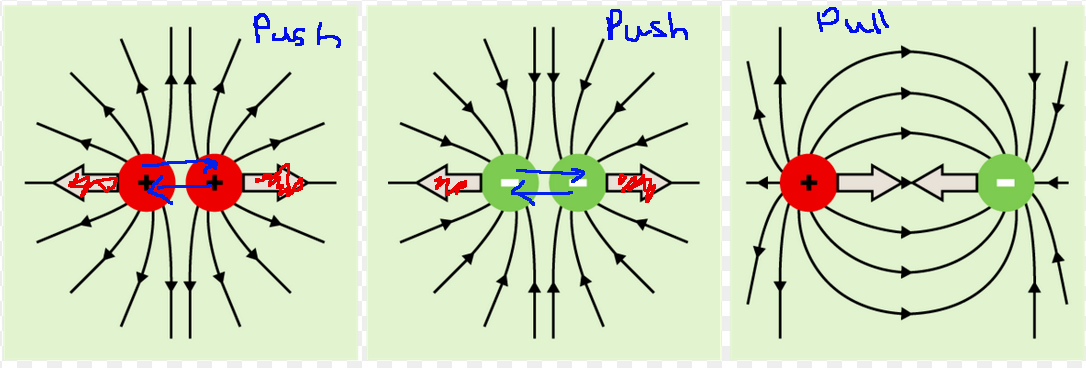
\includegraphics[width=0.9\textwidth]{electric_field_interactions.png}
    \caption{The interaction of electric fields between different charges. The arrows indicate the electrostatic forces exerted on each particle by the other.}
\end{figure}

\subsubsection{Coulomb's Law}

Coulomb's Law is the mathematical formula used to calculate the strength of the electrostatic force between two stationary, electrically charged particles. It describes how much two charges will push or pull each other based on their size and the distance between them.

The law depends on three things:

\begin{itemize}
    \item \textbf{Magnitude of Charge ($q$)}: The more electrical charge the particles have, the stronger the force.
    \item \textbf{Distance ($r$)}: The further apart the particles are, the weaker the force.
    \item \textbf{The Constant ($k$)}: A fixed number (Coulomb's Constant) that represents the strength of the electric force in a vacuum (completely empty space so no air, no atoms, no molecules).
\end{itemize}

The formula is written as:

$$F = k\frac{q_1q_2}{r^2}$$

\begin{itemize}
    \item $F$: The electrostatic force (measured in Newtons).
    \item $k$: Coulomb's Constant ($\approx 8.99 \times 10^9 $ N$\cdot$m$^2$/C$^2$).
    \item $q_1$, $q_2$: The quantity of charge on each particle (measured in Coulombs).
    \item $r$: The distance between the centers of the two charges (measured in meters).
\end{itemize}

The force is directly proportional to the the product of the charges. It is also inversely proportional to the square of the distance meaning that the force weakens rapidly as charges move apart.

\subsubsection{What is a Coulomb?}

A Coulomb (C) is the standard unit used to measure the quantity of electric charge. 1 Coulomb is defined as the total charge of approximately 6.242 quintillion electrons (making the actual total charge negative).

$$1 \; \mathrm{C} \approx 6.242 \times 10^{18} \; \mathrm{electrons}$$

\subsection{Electricity}

\subsubsection{Electrical Current}

\begin{itemize}
    \item Electric current is the total charge that passes through some cross-sectional area per unit time i.e the flow rate of electric charge.
    \item This area is usually a slice through a solid material such as a conductor.
    \item The unit to measure current is Coulombs per second also known as Ampere or \emph{amp} ($1 \; \mathrm{A} = 1 \; \mathrm{C/s}$).
\end{itemize}

\paragraph{Negative Current?}

\subsubsection{Conductors}

A conductor is a material that allows electric current to flow through it easily. In conductors, the outermost electrons in the atoms (called valence electrons) are very loosely bound to their parent atoms.

For example, copper has one valence electron. In a solid block of copper the nuclei of the atoms sit in an organized grid or lattice. However, since the valence electron is so far from its own nucleus, the neighbouring nuclei pull on it just as strongly. As a result these electrons break free and roam throughout the entire piece of metal which leaves behind a rigid structure of positively charged copper ions submerged in a "fluid" of moving negative electrons. However, these free electrons do not travel anywhere in particular and so no current is created.

The copper is held together by the \textbf{electrostatic force}. The positive copper ions want to repel each other however the "sea" of negative electrons flowing between them acts like a powerful atomic glue. The positive ions are strongly attracted (attractive force) to the negative "sea" surrounding them which holds the lattice together in a tight, solid structure.

\begin{figure}[H]
    \centering
    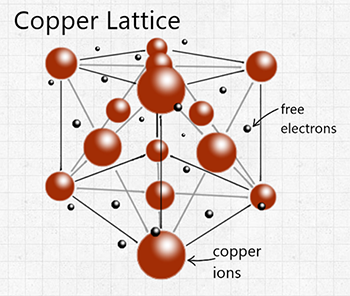
\includegraphics[width=0.5\textwidth]{copper_lattice.png}
    \caption{Illustration of valence electrons moving freely throughout a copper lattice.}
\end{figure}

\subsubsection{Voltage}

Voltage is defined as the eletrical potential difference \emph{between two points}. It is the "push" or "pressure" that causes charges to move through a conductor.

\begin{figure}[H]
    \centering
    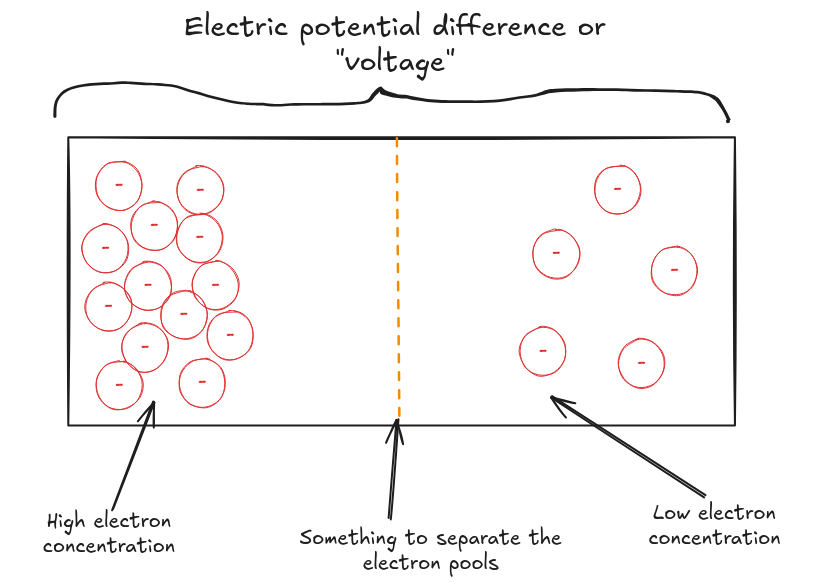
\includegraphics[width=0.8\textwidth]{voltage.png}
    \caption{Illustration of a charge imbalance in a physical medium, producing voltage.}
    \label{fig:voltage}
\end{figure}

Figure \ref{fig:voltage} shows a scenario where voltage exists (between two points). It illustrates a charge imbalance where on the left-hand side of some physical medium there is a high electron concentration and on the right-hand side a low concentration. In the middle there may be something separating them (such as an insulator or an open switch). Due to the high pressure on the left-hand side, there is some arbitrary amount of work that could be done if those electrons were allowed to move to the right hand-side. This is what defines \textbf{potential difference} or \textbf{voltage} and what is measured by voltage. In the event that the electrons were allowed to move, the work done would be a current produced for a brief amount of time across the medium.

If the separator was removed and replaced by a conductive path, the electrons would flow left-to-right until the concentration equalised on both sides, producing an equilibrium in the medium. In this event the "pressure" would be gone and the voltage would drop to \textbf{0V}. The electrons would flow due to the strong electric push force from other electrons behind them. When the equilibrium is reached, all electrons are repelling each other with a similar force and so the net force is zero.

\subsubsection{A Basic Circuit}


\begin{figure}[H]
    \centering
    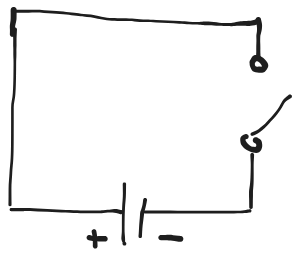
\includegraphics[width=0.3\textwidth]{basic_circuit.png}
    \caption{A basic circuit with a battery and a switch.}
    \label{fig:basic_circuit}
\end{figure}

Consider the circuit in figure \ref{fig:basic_circuit}. The circuit has:

\begin{itemize}
    \item A 9V battery (voltage source).
    \item A switch (a simple gap we can bridge to close the circuit).
    \item Two copper wire conductors (allowing electrons to flow freely amongst them).
\end{itemize}

The battery contains voltage when you compare its positive and negative terminals. A chemical reaction in the battery pumps out electrons from the negative terminal whilst "sucking in" electrons at the positive terminal at the same rate. This builds up the same voltage at the switch as the copper wire between the negative terminal and the switch contains a high concentration of electrons output by the battery. When the circuit is closed, a current is produced and electrons flow around the circuit. The voltage at the battery's negative terminal is continuously 9V and so electrons continuously get pumped out to maintain the current. As a sidenote, the number of electrons flowing through the circuit stays the same.

\end{document}